%!TEX root = ../main.tex
\chapter{Introduction}\label{intro}

% Drafting note: Add citations using keys from the project's .bib file.
% Verify all factual claims against primary literature and project records.

\section{Research Problem and Motivation}\label{sec:research-problem}
    Anthropogenic chemicals enter the environment through industrial activities, agricultural practices, and the manufacture and use of consumer products. These inputs include pharmaceuticals, pesticides, industrial chemicals, and plastic-associated compounds, among other substances. Some chemicals are sufficiently persistent or mobile to move beyond their immediate sources, complicating efforts to determine their distribution and environmental fate~\cite{Manz2023,Blais2015,Wilkinson2022}. Their occurrence is not confined to urban or industrial settings. Investigations of mountain regions and remote waters demonstrate that chemical pollution can be detected far from major emission centers, although the relative contributions of long-range transport and local activities differ among sites~\cite{Daly2005,Xu2011,Ma2025}.

    The analytical problem extends beyond determining whether a sample contains selected contaminants. Environmental samples may produce many signals in liquid chromatography--high-resolution mass spectrometry (LC-HRMS), but detecting a signal does not establish the chemical identity of the substance responsible for it. Traditional targeted measurements are useful when the compounds of interest are known in advance; they are less suited to surveying chemical features that were not anticipated when a method was developed. Suspect screening and non-targeted analysis (NTA) broaden the range of features that can be investigated, yet incomplete reference libraries and uneven spectral coverage continue to constrain identification~\cite{Manz2023,Schulze2020,Hupatz2025}.

    This limitation is especially important for remote environmental samples. A database match may support a candidate assignment for one feature, while nearby features in the same dataset remain unannotated despite containing potentially useful tandem mass spectrometry (MS/MS) information. Molecular networking offers a way to examine these data by representing features as nodes and retaining relationships between features with sufficiently similar MS/MS spectra. The resulting network can help researchers explore candidate chemical relationships and prioritize features for further study, but a network connection is not itself a confirmed molecular identification~\cite{Wang2016,Bittremieux2022,Schymanski2014}.

    The present Senior Independent Study addresses a second, connected problem: the need for a dependable computational workflow through which chemists can construct, inspect, preserve, and interpret molecular networks. For the College of Wooster's environmental HRMS research, useful software must connect the displayed network to the underlying spectral evidence and feature metadata while making its computational decisions reproducible. This project therefore combines environmental chemistry with software engineering. Its central contribution is the development and evaluation of a molecular-networking workflow and interface, using environmental HRMS data as both the motivating application and the basis for chemical case studies.
   
\section{Environmental and Chemical Background}\label{sec:environmental-background}

    \subsection{Long-Range Transport of Organic Contaminants}\label{subsec:long-range-transport}

        % Organic contaminants can move away from their original sources through atmospheric processes. Their movement and deposition depend on properties such as volatility and persistence, as well as environmental conditions. Some semivolatile compounds can undergo repeated cycles of volatilization, atmospheric transport, and deposition, allowing them to reach regions distant from where they were emitted. Temperature gradients and precipitation can influence where these chemicals are deposited.
        % TODO: Support this discussion with primary literature and distinguish
        % established transport mechanisms from processes not measured in this project.

        Once released, an organic chemical's distribution depends on its physicochemical properties, its susceptibility to degradation, and the environmental processes acting on it. Atmospheric transport is one route by which certain pollutants can reach distant ecosystems. Volatilization, emissions associated with combustion or other activities, and the movement of particle-associated compounds can introduce chemicals into the atmosphere. During transport, reactions such as oxidation and photolysis may alter the original substances, producing transformation products with properties that differ from those of their precursors~\cite{Daly2005,Zahn2024}. The presence of a chemical in a remote sample, however, does not by itself establish its source or the pathway by which it arrived.

        For some semivolatile organic compounds (SVOCs), repeated volatilization, atmospheric movement, and redeposition can contribute to long-distance redistribution. This sequence is often described as the \emph{grasshopper effect}. Global fractionation and related temperature-dependent partitioning processes can favor the transfer of certain chemicals toward cooler regions, including mountain environments~\cite{Wania1996,Daly2005}. These mechanisms are particularly relevant to persistent compounds whose transport and deposition can occur over extended timescales. They should not be generalized to every pharmaceutical, pesticide, or other chemical detected by HRMS, because environmental behavior varies substantially among substances.

        Mountain topography and climate influence where transported contaminants are deposited. Orographic precipitation can increase wet deposition as air masses rise and cool, while snowfall can scavenge some gas-phase and particle-associated chemicals. Temperature gradients also affect air--surface exchange and the partitioning of SVOCs among air, snow, vegetation, and other surfaces~\cite{Catalan2015,Herbert2006,Davidson2003}. These processes operate together, rather than as independent explanations for every observation at a mountain site.

        % Figure adapted from the original Junior I.S. manuscript.
        % Confirm permission/attribution requirements before final submission.
        \IfFileExists{figures/imgs/TransportMech.png}{%
        \begin{figure}[htbp]
            \centering
            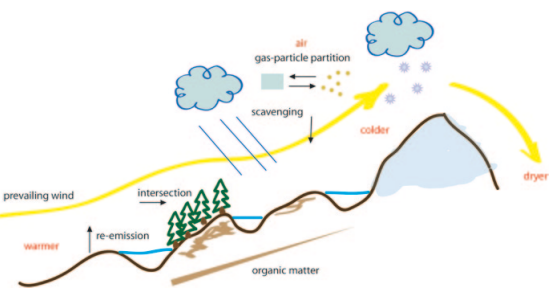
\includegraphics[width=0.82\textwidth]{figures/imgs/TransportMech.png}
            \caption{Conceptual pathways for atmospheric transport and deposition of contaminants in mountainous terrain, including precipitation scavenging, air--surface exchange, and elevation-dependent environmental conditions. Reproduced or adapted from the source discussed by Catalan~\cite{Catalan2015}; confirm the original figure attribution.}
            \label{fig:TransportMechanism}
        \end{figure}
        }{%
        % TODO: Restore figures/imgs/TransportMech.png to display the transport figure.
        }

    \subsection{High-Altitude and Remote Surface-Water Environments}\label{subsec:high-altitude-environments}

        % Remote, high-altitude environments provide useful settings for studying the distribution of environmental contaminants. Locations in the project's research context include Mount Everest, Mount Kilimanjaro, the Qinghai--Tibetan Plateau, and associated surface-water environments. Snow, precipitation, and surface water can provide evidence of atmospheric transport and deposition. Remoteness does not guarantee isolation from human-associated chemicals.
        % This project uses existing environmental HRMS data; sample collection is not itself a contribution of this thesis. The origins, sample types, and analytical details of the datasets used in the software evaluation will be documented in Chapter~2.
        % TODO: Add findings and citations from primary studies relevant to the actual
        % datasets. Do not imply that every cited location is represented in the data.

        High-altitude regions offer valuable settings for examining contaminant transport because their climatic conditions can favor deposition, seasonal storage, and subsequent redistribution of chemicals. Mountain snow and ice may temporarily retain atmospheric contaminants, and melting can transfer some of these substances into downstream waters. The timing and magnitude of release depend on snowpack processes and the properties of the chemicals involved~\cite{Herbert2006,Meyer2008}. Such pathways matter for interpreting surface-water samples, but the detection of a feature alone does not establish its ecological effect or the extent of exposure to organisms.

        Research on mountainous environments has documented persistent organic contaminants and other human-associated chemicals in regions that are geographically distant from major industrial centers~\cite{Daly2005,Xu2011,WangCong2019}. Studies of the Qinghai--Tibetan Plateau also illustrate that spatial patterns of contamination can be influenced by human activity within a highland basin, not solely by long-range atmospheric transport~\cite{Ma2025}. Consequently, these environments should be treated as chemically informative rather than assumed to be free of local sources. Tourism, settlement, transportation, and regional activities may contribute alongside atmospheric inputs, depending on the location and compound.

        Cold trapping is one explanation for the accumulation of particular semivolatile contaminants in mountainous environments. As air temperatures decrease with elevation, some compounds partition more readily into cooler environmental compartments. Seasonal changes can then modify the balance between deposition and re-emission. These exchanges provide a conceptual explanation for how contaminants can be redistributed; they are not direct measurements of the samples analyzed in this thesis~\cite{Daly2005,Herbert2006}.

        \IfFileExists{figures/imgs/Daly_SVOCs.png}{%
        \begin{figure}[htbp]
            \centering
            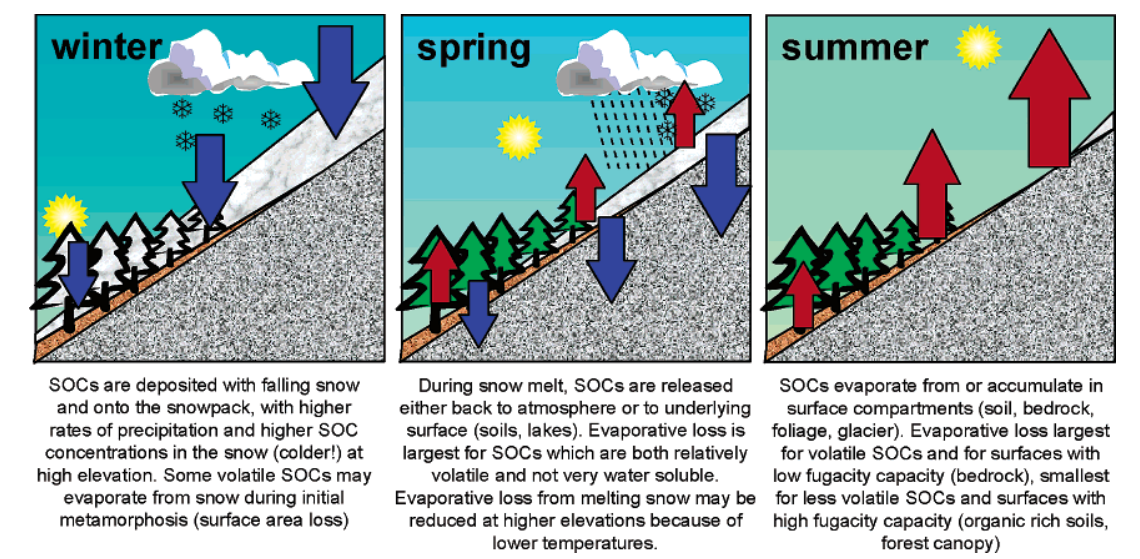
\includegraphics[width=0.78\textwidth]{figures/imgs/Daly_SVOCs.png}
            \caption{Illustration of seasonal air--surface exchange processes affecting semivolatile organic contaminants along a mountain slope. From the discussion of organic contaminants in mountains by Daly and Wania~\cite{Daly2005}; verify reproduction or adaptation permissions.}
            \label{fig:AirSurfaceExchange}
        \end{figure}
        }{%
        % TODO: Restore figures/imgs/Daly_SVOCs.png to display the seasonal exchange figure.
        }

        The published mountain literature provides context for the environmental samples considered in this project. Daly and Wania reviewed studies of persistent organic contaminants at mountain locations and the factors affecting their transport and retention~\cite{Daly2005}. The compilation previously reproduced in the Junior I.S. as a figure is useful as evidence of the range of mountain sites and chemical classes investigated; it should not be described as a plot of contaminant concentrations because it summarizes studies and sampling information rather than presenting a common quantitative scale.

        \IfFileExists{figures/imgs/DalyData.png}{%
        \begin{figure}[htbp]
            \centering
            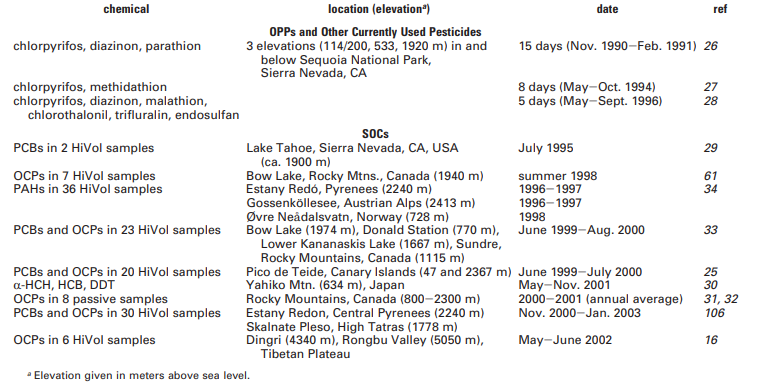
\includegraphics[width=0.92\textwidth]{figures/imgs/DalyData.png}
            \caption{Summary of selected mountain-air contaminant investigations, including reported chemical classes, study locations, and sampling periods, as compiled by Daly and Wania~\cite{Daly2005}. This is a study-summary table, not a comparison of measured concentrations. Verify the original figure attribution.}
            \label{fig:MountainStudies}
        \end{figure}
        }{%
        % TODO: Restore figures/imgs/DalyData.png to display the mountain study summary.
        }

        The present project is motivated by environmental HRMS datasets associated with remote and high-altitude locations, including the Himalayas, Mount Kilimanjaro, and the Qinghai--Tibetan Plateau. These locations provide a chemical context in which both previously recognized contaminants and unannotated features are of interest. The exact samples, matrices, collection locations, and data subsets included in the software evaluation will be specified in Chapter~2. No claim is made here that every location mentioned in the literature is represented in the dataset used for the final case studies.

    \subsection{Previous Wooster Research and the Identification Gap}\label{subsec:wooster-research-gap}

        % Previous research associated with the College of Wooster has investigated organic contaminants in remote and high-altitude environmental samples. This work provides the chemical and analytical context for the current project. Even when LC-HRMS detects features of interest, not every feature can be assigned confidently to a specific compound. A feature may have accurate-mass, retention-time, isotope, or MS/MS information without a confirmed chemical identity.
        % The gap is both chemical and computational. Chemically, researchers need ways to prioritize and interpret features that lack confident identifications. Computationally, they need tools that allow spectral relationships and associated metadata to be examined consistently. This thesis addresses the computational part of that problem while using environmental data to demonstrate how the workflow can support chemical investigation.
        % TODO: Cite specific Wooster studies and distinguish prior researchers' work
        % from analyses performed as part of this thesis.

        Previous work associated with the College of Wooster provides a direct foundation for this study. Fan's undergraduate research investigated suspect screening and semi-quantification of organic contaminants in snow and water from the Qinghai--Tibet Plateau and other high-mountain regions~\cite{Wenkai}. Related research involving Wooster investigators has applied LC-HRMS suspect screening to pesticides in rain and snow, as well as NTA and suspect screening to organic contaminants in temperate snowfall~\cite{Gray2022,NinoSuastegui2025}. These studies are not interchangeable: the temperate precipitation investigations demonstrate analytical approaches, while Fan's work is more directly connected to the remote high-altitude samples motivating this project.

        The identification gap arises because feature detection can yield more information than reference-based annotation can explain. Accurate mass, retention time, isotope information, and MS/MS spectra can be available for a detected feature even when its chemical structure remains uncertain. An unannotated feature may represent a chemical absent from the library, a feature with insufficient-quality evidence, or another analytical signal requiring additional interpretation. It should not automatically be described as a new contaminant or a transformation product~\cite{Manz2023,Schulze2020,Schymanski2014}.

        This distinction defines the need for both chemistry and computer science in the current work. From the chemistry perspective, researchers need to organize evidence and prioritize features that merit further investigation. From the computational perspective, they need to calculate spectral relationships consistently, retain the information behind those relationships, and navigate the resulting network without losing the connection to the original data. The purpose of the new software is to support this investigative process, not to replace confirmatory chemical analysis.

\section{LC-HRMS, Suspect Screening, and Non-Targeted Analysis}\label{sec:lc-hrms}

    \subsection{LC-HRMS and Tandem Mass Spectrometry}\label{subsec:lc-hrms-msms}

        % Liquid chromatography separates components of a sample before they enter a mass spectrometer. High-resolution mass spectrometry measures ions with high mass accuracy and provides information used to characterize molecular features. In tandem mass spectrometry (MS/MS), selected precursor ions are fragmented and the resulting product-ion spectra provide additional evidence about molecular structure. These data support chemical annotation and comparison, but their interpretation depends on data quality and available reference information.
        % TODO: Describe the actual instrument, chromatography, ionization modes, and
        % acquisition conditions in Chapter 2 after checking laboratory records.

        Liquid chromatography separates components of a sample before mass-spectrometric detection, helping resolve some of the complexity of environmental mixtures. High-resolution mass spectrometry measures ions with sufficient mass accuracy to support candidate elemental compositions and other forms of chemical investigation. Depending on the acquisition and processing methods, an LC-HRMS feature can be characterized by a mass-to-charge ratio ($m/z$), retention time, signal intensity, and additional evidence such as an isotope pattern. These attributes are useful for organizing a dataset, but they do not necessarily determine a unique chemical structure~\cite{Manz2023,Kind2018}.

        Tandem mass spectrometry provides another source of information by selecting precursor ions and recording the product ions generated during fragmentation. MS/MS patterns can assist in distinguishing candidates, comparing features, and searching spectral libraries. Their interpretation depends on acquisition conditions, spectral quality, and the reference data available for comparison~\cite{Kind2018,Hupatz2025}. The specific LC-HRMS instrumentation, ionization modes, acquisition strategy, and upstream processing steps associated with the datasets used in this thesis are documented in Chapter~2 rather than assumed from the general analytical literature.

    \subsection{Molecular Features Versus Identified Compounds}\label{subsec:features-compounds}

        % A molecular feature is an observed signal characterized by analytical attributes such as mass-to-charge ratio, retention time, and, when available, isotope or MS/MS information. A feature should not automatically be treated as a confirmed compound. Adduct formation, in-source fragmentation, isomers, incomplete spectra, and limited reference information can complicate interpretation.
        % This thesis uses the term \emph{feature} for detected signals whose chemical identities have not been confirmed. The term \emph{compound} is reserved for cases where the evidence supports that terminology. Network connections and candidate annotations are evidence to investigate, not substitutes for appropriate chemical confirmation.

        A \emph{molecular feature} is an analytical observation rather than a confirmed chemical identity. Multiple observed signals can arise from a single substance through different adducts, isotopes, or fragments, while different substances can also produce overlapping or difficult-to-distinguish signals. For this reason, a feature count is not equivalent to a count of unique contaminants. Likewise, a spectral library match or a relationship to an annotated neighbor does not automatically justify calling an unknown feature an identified compound~\cite{Manz2023,Schymanski2014}.

        Confidence in a chemical assignment should be communicated in relation to the supporting evidence. Schymanski and colleagues proposed a framework for reporting confidence levels in HRMS-based small-molecule identification, ranging from confirmed structures to less specific candidate or formula-level information~\cite{Schymanski2014}. Within this thesis, \emph{feature} is used when identity has not been established, while \emph{candidate annotation} or \emph{tentative identification} describes an assignment supported by incomplete evidence. A confirmed identification requires the appropriate confirmation criteria, such as comparison with an authentic reference standard when relevant. The confidence associated with individual case-study features will be stated rather than inferred from network appearance.

    \subsection{Suspect Screening and Non-Targeted Analysis}\label{subsec:suspect-nta}

        % Targeted analysis focuses on a predefined set of compounds. Suspect screening examines data for compounds on a suspect list, including compounds that may not be part of a conventional targeted method. Non-targeted analysis (NTA) aims to detect and investigate a broader range of chemical features without restricting the analysis to a fixed list of target compounds.
        % These approaches are complementary. Suspect screening can investigate compounds for which there is a prior reason to look, while NTA can retain information about features not anticipated in advance. Neither approach guarantees that every detected feature can be identified. Candidate assignments must be evaluated against available mass, retention-time, isotope, and fragmentation evidence, as applicable.

        Targeted analysis begins with a defined set of analytes and methods selected to measure them. It is valuable for questions concerning known chemicals, but its scope is constrained by the compounds included in the method. Suspect screening broadens that scope by examining acquired data for chemicals of prior interest, often using information from candidate lists and available analytical evidence. NTA takes a wider approach by retaining and investigating features without requiring that every candidate be specified before data acquisition~\cite{Manz2023,Schulze2020}.

        These strategies are complementary rather than mutually exclusive. Suspect screening can prioritize features associated with known environmental concerns, while NTA can reveal additional signals that do not match the current suspect list. Published studies of pesticides in rain and snow and of broader organic chemical mixtures in snowfall demonstrate the value of these approaches in environmental LC-HRMS workflows~\cite{Gray2022,NinoSuastegui2025}. At the same time, an expanded set of detected features creates a larger interpretation problem: researchers must decide which signals are chemically meaningful and what evidence supports each possible assignment.

        The term \emph{exposome} provides a broader context for this challenge by referring to the totality of exposures across time, including chemical exposures. NTA and suspect screening can contribute information about portions of this chemical landscape, but no single analytical dataset measures the entire exposome~\cite{Manz2023}. For the present project, the more immediate objective is to investigate environmental feature relationships in the available data, not to quantify total exposure or infer health effects.

    \subsection{Limitations of Current Identification Approaches}\label{subsec:identification-limitations}

        % Reference databases and spectral libraries are incomplete. A detected feature may not have a suitable reference spectrum, and different structures can sometimes produce similar or partially overlapping fragmentation patterns. Data quality, acquisition conditions, and processing choices can also affect the evidence available for interpretation.

        % Identifying and prioritizing unknown features therefore requires researchers to combine different types of evidence and preserve uncertainty in their conclusions. A computational tool can help organize data and make relationships easier to inspect, but it should not convert a similarity score or network connection into an unsupported claim of chemical identity.
        Even when high-resolution data are available, many features remain without confident annotations. Reference databases may not contain a relevant chemical or its spectrum, experimental conditions may differ from those used to generate a library spectrum, and the available MS/MS data may be incomplete or ambiguous. Reviews of environmental NTA and computational structural annotation describe these constraints and emphasize the importance of quality control and careful reporting~\cite{Schulze2020,Hupatz2025,Fisher2022}.

        The consequence is a gap between \emph{detection} and \emph{interpretation}. Increasing the number of observed features does not necessarily increase the number of confidently identified substances. Additional computational methods can help organize the evidence, identify promising comparisons, and prioritize follow-up work, but they must preserve uncertainty instead of presenting every computational association as a chemical conclusion. Molecular networking is one such method, and its theoretical basis is developed in the following section.

\section{Molecular Networking and Theoretical Foundations}\label{sec:molecular-networking}

    \subsection{MS/MS Fragmentation and Spectral Similarity}\label{subsec:fragmentation-similarity}

        % MS/MS spectra represent product ions generated when a precursor ion fragments under specified conditions. Related molecules may share some fragments or fragmentation patterns, so comparing spectra can provide clues about structural similarities. The strength of these inferences depends on spectrum quality, the comparison method, and the chemical context.
        % Spectral similarity is best treated as a way to prioritize and explore possible relationships. It is not, on its own, definitive evidence that two features represent the same molecule or lie on a specific transformation pathway.

        A tandem mass spectrum records product ions and their intensities after a precursor ion undergoes fragmentation. Structurally related molecules can share fragments or fragmentation pathways, which creates a basis for comparing their spectra. Nevertheless, the relationship between structure and spectral similarity is not one-to-one. Different compounds may share characteristic fragments, and the same compound may yield different relative intensities under different acquisition conditions. Spectral comparisons are therefore useful evidence for exploratory analysis, not direct proof of identity~\cite{Wang2016,Bittremieux2022}.

        In a molecular network, this comparison becomes a relationship between features. An annotated feature may provide context for neighboring features, including those that have no direct library match. Such proximity can help prioritize a chemical family or candidate structure for further investigation, but any proposed relationship must be evaluated against the available fragmentation data, precursor information, and independent chemical evidence~\cite{Schmid2021,Ernst2019,Schymanski2014}.

    \subsection{Cosine Similarity and Molecular-Network Construction}\label{subsec:cosine-network}

        % A spectral similarity score quantifies the correspondence between two spectra under a specified comparison procedure. Cosine similarity is one common approach. After spectra are represented and peaks are matched according to defined rules, the score summarizes alignment between the resulting spectral vectors. The score depends on implementation choices such as peak matching, mass tolerances, preprocessing, and filtering.
        % In a molecular network, each node represents a molecular feature and an edge represents a relationship that meets the selected similarity criteria. Edge weights or labels can retain the similarity score so researchers can inspect the computational relationship. Thresholds affect the resulting graph: stricter criteria may remove weaker connections, while more permissive criteria may create a denser network. The chosen settings and their rationale should therefore be documented.
        % TODO: Add the exact similarity implementation, peak-matching rules, and
        % thresholds once finalized. Detailed implementation belongs in Chapter 2.

        Cosine similarity is a common method for measuring agreement between represented mass spectra. After an appropriate peak-matching or alignment procedure, spectra can be expressed as nonnegative intensity vectors $\mathbf{x}$ and $\mathbf{y}$. Their cosine similarity is
        \begin{equation}
            \operatorname{cos}(\mathbf{x},\mathbf{y})
            = \frac{\mathbf{x}\cdot\mathbf{y}}
            {\lVert\mathbf{x}\rVert_2\,\lVert\mathbf{y}\rVert_2}.
            \label{eq:spectral-cosine}
        \end{equation}
        For nonnegative intensity vectors, values closer to one indicate greater agreement under the selected representation and matching procedure. The score is meaningful only in the context of those choices. Peak matching, mass tolerances, intensity treatment, minimum matching requirements, and any modified-cosine or neutral-loss logic can change the comparisons and the resulting network~\cite{Bittremieux2022,DallaValle2025}.

        The score is not itself an edge. A molecular-networking workflow applies additional rules to determine which pairwise similarities are retained as connections, such as a minimum score or other filters. Different rules can produce different network densities and connected components from the same spectra. Consequently, a reproducible workflow must document its comparison method and parameter values. Chapter~2 describes the actual algorithm and edge-selection rules implemented in this project; Equation~\ref{eq:spectral-cosine} establishes the general mathematical foundation rather than claiming that a particular implementation has already been validated.

    \subsection{Graph Theory: Nodes, Edges, and Connected Components}\label{subsec:graph-theory}

        % Graph theory provides a formal way to represent relationships among objects. In molecular networking, nodes represent features and edges represent the spectral relationships retained by the workflow. A connected component is a set of nodes connected through paths in the graph. Isolated nodes have no retained edges under the selected network criteria.
        % These structures help summarize and navigate relationships in a dataset. However, a connected component should not automatically be interpreted as one chemical family, and an edge should not be treated as proof of shared identity or a reaction pathway. Interpretation requires considering the graph alongside spectral evidence, metadata, annotations, and analytical limitations.

        A molecular network can be represented as a graph $G=(V,E)$, where $V$ is the set of nodes representing analytical features and $E$ is the set of retained spectral relationships. An edge may carry a similarity score or other metadata describing the evidence for the relationship. This representation provides a computational structure for organizing large sets of pairwise comparisons and exploring groups of related observations~\cite{Barabasi2016,Wang2016}.

        A \emph{connected component} is a maximal set of nodes linked through paths in the graph. Components can help organize a network into smaller groups for inspection, while isolated nodes represent features without retained edges under the chosen criteria. These are graph properties, not chemical classifications. In particular, two features in the same component may be connected only indirectly, and membership in a component does not establish a shared molecular formula, common source, or transformation pathway.

    \subsection{Network Visualization and Interpretation}\label{subsec:network-visualization}

        % Network visualization can help researchers inspect complex relationships that may be difficult to explore in a table alone. Selecting nodes and edges, viewing feature metadata, examining similarity values, and filtering the network can connect the overall graph to the underlying chemical evidence. Visual encodings should communicate meaningful properties without implying more certainty than the data support.
        % The interface is most useful when users can move between the network-level view and the evidence behind a connection. Users should be able to inspect which features are connected, why an edge is present under the selected criteria, and what information is available about the features. Important settings and data provenance should be accessible enough to support repeatable analysis.

        Visualization translates the graph into an interface that chemists can explore. A useful view should allow researchers to identify features and their connections, inspect similarity scores, and retrieve the metadata or spectra associated with a selected node or edge. Color, size, layout, and filtering can make patterns easier to see, but these visual choices must be defined so that they do not imply greater chemical certainty than the underlying data justify. Research on interactive graph exploration supports the importance of connecting overview visualizations with inspectable data and user tasks~\cite{Pienta2015,Jacomy2014}.

        The distinction between a graphical display and a scientific workflow is important for this project. A static image of a network may communicate broad structure, but it cannot by itself establish which source records produced an edge or whether an analysis can be repeated with the same parameters. The proposed interface therefore emphasizes the relationship between visual elements, underlying feature data, and the computations used to generate connections. The implemented interactions and their evaluation will be described in Chapters~2 and~3.

    \subsection{Limitations of Spectral Similarity as Evidence of Chemical Identity}\label{subsec:spectral-limitations}

        % A high spectral similarity score indicates agreement under the selected computational comparison; it does not independently establish molecular identity. Similar spectra can arise for different structures, and structurally related compounds can produce different spectra under different conditions. Missing or low-quality MS/MS data may also weaken or prevent meaningful comparisons.
        % The software developed in this project is intended to support exploration of evidence rather than replace expert chemical judgment or confirmatory experiments. Where reference standards or other appropriate confirmation are absent, the thesis will distinguish tentative annotations and possible relationships from confirmed identifications.

        Spectral similarity can support hypotheses about structural relationships, but it cannot independently confirm the identity of an unknown compound. Shared fragment ions may arise from different structures, and changes in collision energy, ionization, and spectral quality can alter the apparent similarity between spectra~\cite{Bittremieux2022,Hupatz2025}. Likewise, a mass difference between two connected features does not, without further evidence, demonstrate that one is a transformation product of the other.

        This limitation shapes both the software design and the chemistry case studies. The network should make comparisons inspectable and preserve annotation confidence, while interpretation should distinguish observations, tentative hypotheses, and confirmed assignments. The intended benefit is more informed prioritization of unknown features, not an automatic conversion of spectral relationships into definitive chemical identifications~\cite{Schymanski2014,Chao2025}.

\section{Existing Software and Research Gap}\label{sec:existing-software}

    \subsection{MS-DIAL and GNPS in the Existing Workflow}\label{subsec:msdial-gnps}

        % The existing research workflow uses MS-DIAL for upstream processing of mass-spectrometry data and molecular-networking tools such as the Global Natural Products Social Molecular Networking platform (GNPS) to explore spectral relationships. These tools address different stages of the workflow: processing software prepares and organizes analytical data, while molecular-networking software represents relationships among features.
        % This project builds on that workflow rather than assuming that any one tool is universally unsuitable. The relevant question is whether the workflow used for the College of Wooster's environmental HRMS research meets practical requirements for data handling, network inspection, reproducibility, and interpretation.
        % TODO: Verify tool versions, export formats, and workflow steps against
        % project records. Describe only limitations that were observed or documented.

        Mass-spectrometry analysis typically involves multiple computational stages. In the Wooster research context, MS-DIAL is used for upstream data processing and feature-level outputs, while molecular-networking approaches associated with the Global Natural Products Social Molecular Networking platform (GNPS) provide methods for organizing MS/MS relationships~\cite{Tsugawa2015,Wang2016,Schmid2021}. These tools address different analytical tasks and have established value in their respective areas. The objective of this thesis is not to suggest that the existing platforms are universally inadequate, nor to replace every stage of LC-HRMS data processing.

        Instead, the project focuses on the transition from processed analytical data to a molecular network that can be explored and reproduced in the local research workflow. The input and export formats, metadata requirements, and comparison methods at this boundary affect whether the results remain interpretable after they leave the original processing software. The specific versions and settings used for the project data will be documented in Chapter~2.

    \subsection{Documented Limitations in the Wooster Research Workflow}\label{subsec:workflow-limitations}

        % The motivation for this project includes workflow difficulties reported during local molecular-networking work, particularly around preserving work and reliably saving or exporting results. These concerns should be described as observed or reported issues in this specific research context, not as a general claim that GNPS or other existing platforms fail for all users.
        % The project will translate relevant research needs into explicit software requirements. These may include dependable input handling, inspectable node and edge information, links between network elements and chemical metadata, and clear behavior when saving or exporting results. The final requirements should reflect documented needs and features actually implemented and evaluated.

        The software-development motivation arose from difficulties reported in local molecular-networking work, particularly around saving, retaining, or exporting analyses and results. Such problems matter because a network is useful for research only when its underlying data, parameter choices, and interpretations can be revisited. These concerns are presented as local workflow requirements that motivate this project, not as evidence that GNPS necessarily behaves the same way for every user or deployment.

        A reliable workflow must also support the scientific interpretation of its outputs. A chemist examining a connected pair of features needs access to the corresponding identifiers, spectra, annotations, and similarity evidence. Without those links, an attractive visualization may be difficult to verify or use in subsequent analysis. Reproducibility likewise depends on retaining input provenance, computational parameters, and sufficient documentation to repeat the workflow~\cite{Wilson2017,Pienta2015}. The particular requirements adopted for this project will be made explicit and evaluated rather than assumed to have been satisfied.

    \subsection{The Need for Software Designed Around Chemists' Needs}\label{subsec:chemist-centered-software}

        % Molecular-networking software must do more than generate a graph. It should help users move between a network-level view and the underlying evidence, understand how connections were calculated, and preserve the information needed to reproduce an analysis. The interface should make important details accessible without requiring users to reconstruct the workflow from separate files or undocumented steps.
        % This project treats software reliability and usability as research concerns alongside the chemical application. The proposed contribution is a workflow and interface tailored to the current environmental HRMS research context, evaluated through computational tests and case studies using real data. Its success will be assessed based on implemented functionality and measured results rather than assumed in advance.

        The research gap is therefore both analytical and computational. Incomplete reference coverage leaves many environmental HRMS features unidentified, while a practical molecular-networking workflow must make spectral comparisons, graph relationships, and supporting metadata accessible to researchers. Existing tools demonstrate the value of molecular networking, but the requirements of a particular laboratory workflow still need to be defined, implemented, and tested~\cite{Wang2016,Schmid2021,Chao2025}.

        This thesis approaches software as a scientific research instrument rather than merely a way to display a network. The proposed contribution is a workflow and interface tailored to Wooster's environmental HRMS context, with attention to computational correctness, reproducibility, data handling, and the interpretability of network relationships. Its value will be assessed through software evaluation and chemical case studies. The chemistry contribution concerns what can reasonably be learned or prioritized from the environmental data; the computer science contribution concerns how reliably and transparently the software supports that investigation.

\section{Research Question and Specific Aims}\label{sec:research-question}

    The central research question is:

    \begin{quote}
    What computational workflow and interface are needed to make molecular networking reliable, reproducible, and useful for Wooster's environmental HRMS research?
    \end{quote}

    The project addresses this question through four aims:

    \begin{enumerate}
        \item \textbf{Define the chemistry and data requirements.} Identify the analytical data, metadata, and evidence needed to construct and interpret molecular networks for the environmental HRMS research context.
        \item \textbf{Develop an end-to-end molecular-networking workflow.} Implement a workflow that processes supported input data, compares MS/MS spectra, constructs a network, and allows users to inspect network elements and associated chemical information.
        \item \textbf{Evaluate computational correctness, reproducibility, performance, and workflow usefulness.} Test calculations, input handling, graph construction, repeatability, performance, and relevant user-facing tasks using documented evaluation methods.
        \item \textbf{Apply the software to environmental HRMS case studies.} Use selected environmental data to examine annotated and unidentified features, describe relationships supported by the evidence, and identify remaining uncertainties.
    \end{enumerate}

\section{Project Scope and Thesis Contributions}\label{sec:scope-contributions}

    \subsection{Project Scope}\label{subsec:project-scope}

        This project focuses on computational support for molecular networking using existing environmental HRMS data. It includes defining data requirements, implementing and testing the network workflow, designing an interface for inspecting features and spectral relationships, and applying the software to selected chemical case studies. The specific input formats, data-processing assumptions, software features, and evaluation procedures will be defined in Chapter~2.

        The project does not assume that a network alone can confirm the identity of unknown compounds, prove chemical transformation pathways, or replace reference standards and other confirmatory methods. Software development alone also does not establish the environmental source, toxicity, or ecological effect of a detected feature. Claims in the chemical case studies will be limited to what the available analytical data and supporting evidence justify.

    \subsection{Expected Computer Science Contributions}\label{subsec:cs-contributions}

        The Computer Science contribution is the design, implementation, and evaluation of a molecular-networking workflow and interface for the stated research context. The contribution will be documented through the software architecture, similarity and graph-construction methods, interface behavior, input validation, testing, and reproducibility practices. Chapter~3 will report what was implemented and how it performed under the evaluation procedures.

    \subsection{Expected Chemistry Contributions}\label{subsec:chemistry-contributions}

        The Chemistry contribution is the application of the workflow to environmental HRMS data to investigate spectral relationships among annotated and unidentified molecular features. The case studies will describe the evidence available for selected features, explain how network relationships may help prioritize further investigation, and state the remaining limitations. Tentative network relationships will not be presented as confirmed chemical identifications.

    \subsection{Organization of the Thesis}\label{subsec:thesis-organization}

        Chapter~2 describes the research design, environmental datasets and analytical methods, upstream processing, software requirements and implementation, network construction, and evaluation procedures. Chapter~3 presents the dataset summary, software implementation results, computational validation, performance and workflow evaluation, network characteristics, and chemical case studies. Chapter~4 interprets the computational and chemical findings, discusses design trade-offs and limitations, and considers implications for future environmental HRMS research. Chapter~5 summarizes the contributions, answers the central research question, and identifies future directions.
